\chapter{開発手法}
\label{chap:coding}

本章ではDreamtravelerの概要、利用方法、システム概要について述べる。

\section{概要}
 現在、拡張現実を体験すべくOculous Riftなどのヘットマウントディスプレーをはじめとして様々なツールが開発されている。そこで本研究では睡眠中の夢を自由にコントロールする方法があれば誰もがより簡単に拡張現実を体験をすることができるのではないかと考えた。そこで眠っっている時にその人が過去に体験したことと関連した音を流すことで、その音に基づいて夢を見ることを促進するスマートフォンアプリDreamtravelerを試作した。\\
 Dreamtravelerのターゲットユーザーは日々のストレスから解放されたい人、懐かしい思い出をもう一度体験したい人、物理的に会えない人と会いたい人などが含まれる。\\
 Dreamtravelerには3つ主要な機能がある。一つ目は寝る前に印象に残っている記憶に関する写真と映像を表示する機能。二つ目は睡眠中にREM睡眠を検出し、記憶を連想させる音を流す機能。例えば特別な誰かを連想する音、旅行中によく聞いていた曲、最寄り駅の音楽、好きな映画のサウンドトラックなどだ。三つ目は起床後に夢について記録する夢日記機能である。ユーザーには睡眠前にスマートフォンを画像\ref{DreamtravelerImage}のように枕の横に置いてもらう。\\
 Dreamtravelerは開発途中でまだAppストアには掲示していないが、githubからソースコードを入手することができる。iOSスマートフォンを持っていて、Apple Developerの登録をしている人であればインストールできるようになっている。

\begin{figure}[htbp]
\begin{center}
\includegraphics[width=14cm]{eps/dreamDate02.eps}
\caption{Dreamtraveler:枕の横に配置して、ユーザの体動を観測する}
\label{DreamtravelerImage}
\end{center}
\end{figure}

\section{利用方法}
 ユーザーには予め記憶を思い起こさせる音を登録してもらう。音選びは適している音声と適さない音声があるため注意する必要がある。使用してはいけない音は人の声だ。特に喋りかけてくるような内容の音声は、ユーザーを起こしてしまう可能性が高いということが実験結果から分かった。詳しくは第6章で述べる。逆に適している音は繰り返しある環境下で聞いていた音である。
 アプリの起動後、\ref{le01}のような画面が表示される。そこには「自動ロック機能をOFFにする」「音量は1〜3に設定する」やiPhoneの置く位置などの指示が書かれている。次に\ref{le02}の画面に遷移し、ユーザーの思い出に関連性のある画像を表示する。ここでは寝る前に記憶の情景を思い出す機会を与えている。そして\ref{le03}の画面では思い出の音楽が流れる。音楽を聴きながら、旅先での空間、香り、音の細部までを思い出して、気持ちを落ちつかせて瞑想状態に入ってもらう。次に\ref{le04}の画面に移動する。ユーザーは寝る前にアプリを起動してスタートボタンを押し、起動させたままスクリーンを伏せて枕の横に置く。20〜30分間後にDreamtravelerの加速度が起動をし一晩中ユーザーの体動のトレッキングが行われ、REM睡眠を検知すると音楽がなる。起床後\ref{le05}の画面で、ユーザーは起床すると夢の内容を忘れないように日記に投稿する。

\begin{figure}[htbp]
 \begin{minipage}{0.45\hsize}
  \begin{center}
   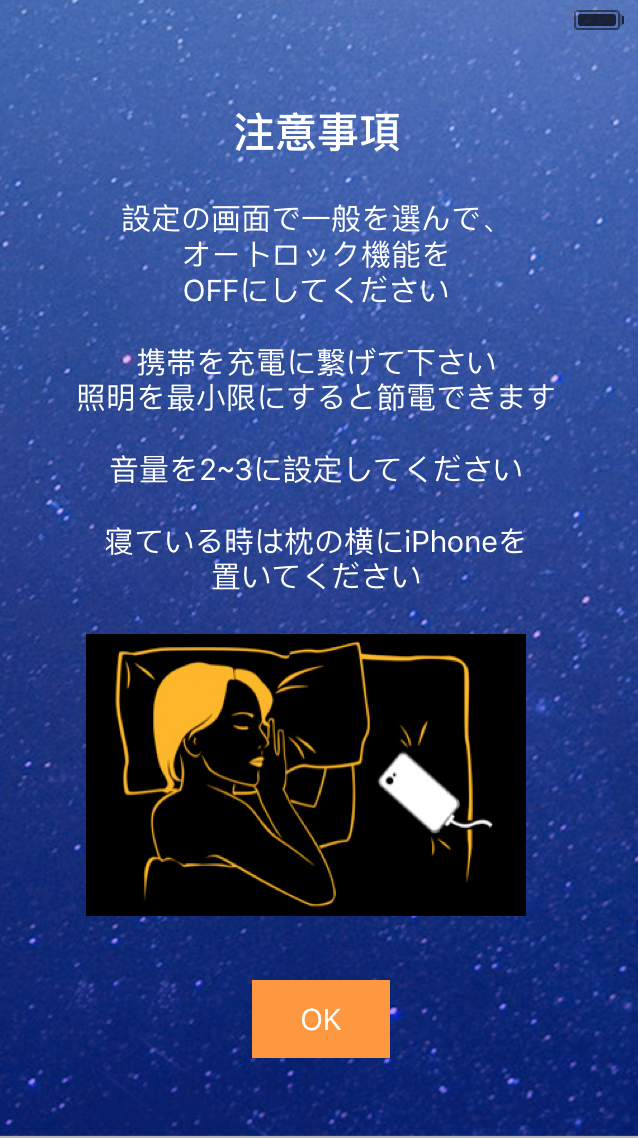
\includegraphics[height=90mm]{eps/AppIntro.eps}
  \end{center}
  \caption{起動画面}
  \label{le01}
 \end{minipage}
 \begin{minipage}{0.45\hsize}
  \begin{center}
   \includegraphics[height=90mm]{eps/AppMemoryImages.eps}
  \end{center}
  \caption{思い出の画像を表示}
  \label{le02}
 \end{minipage}
\end{figure}

\begin{figure}[htbp]
 \begin{minipage}{0.45\hsize}
  \begin{center}
   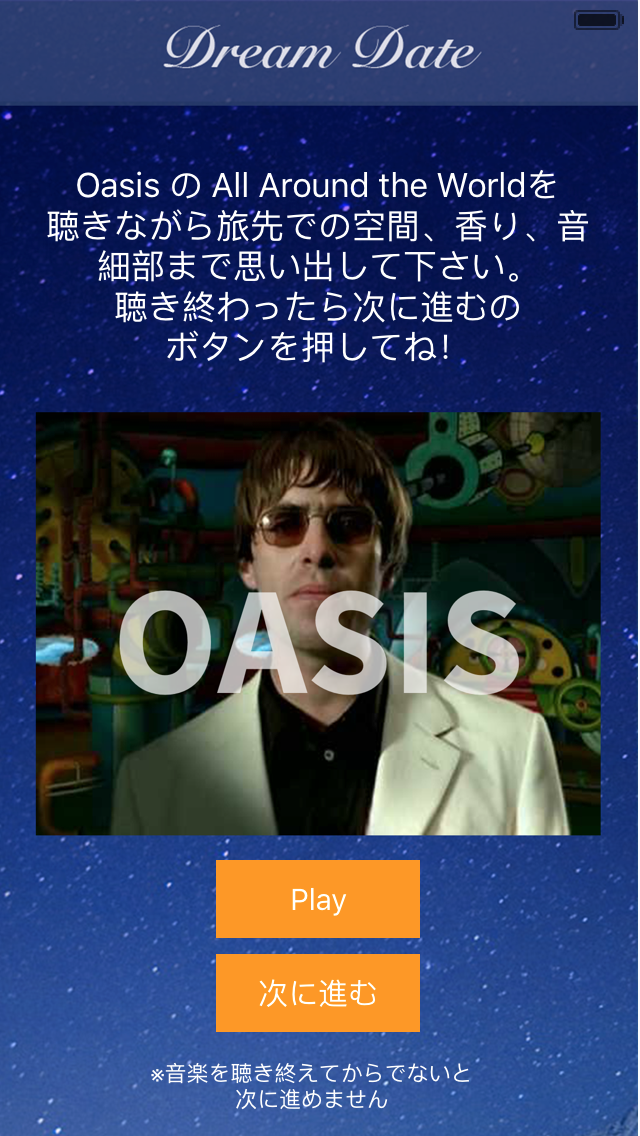
\includegraphics[height=90mm]{eps/AppMusicPlay.eps}
  \end{center}
  \caption{思い出の音楽が流れる}
  \label{le03}
 \end{minipage}
 \begin{minipage}{0.45\hsize}
  \begin{center}
   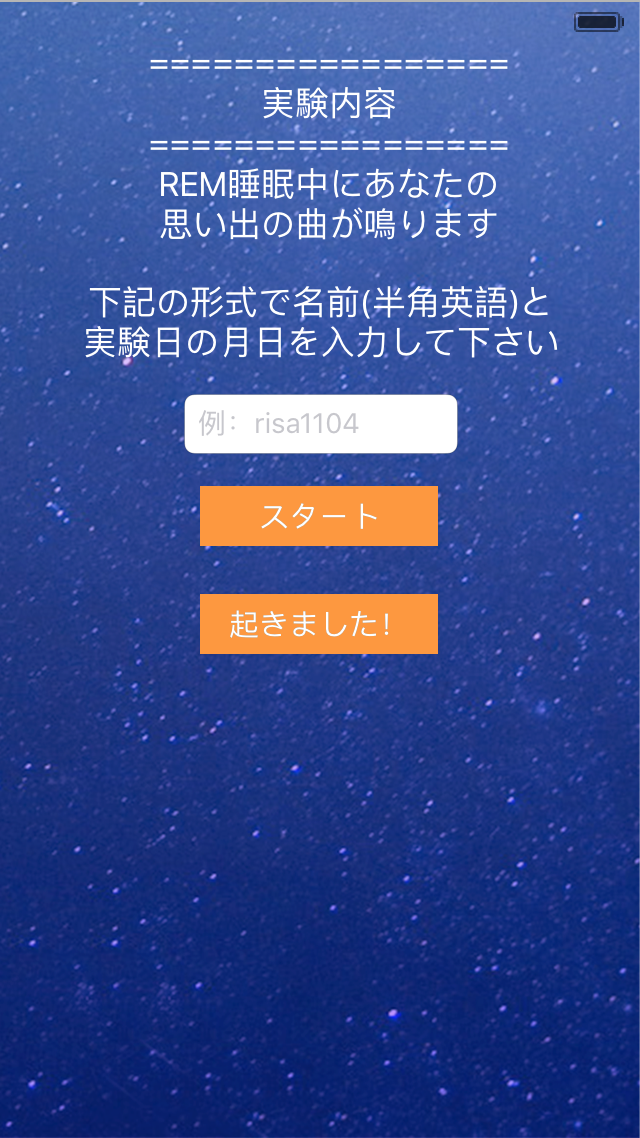
\includegraphics[height=90mm]{eps/AppStart.eps}
  \end{center}
  \caption{眠り開始ボタン}
  \label{le04}
 \end{minipage}
\end{figure}

\begin{figure}[htbp]
 \begin{minipage}{0.45\hsize}
  \begin{center}
   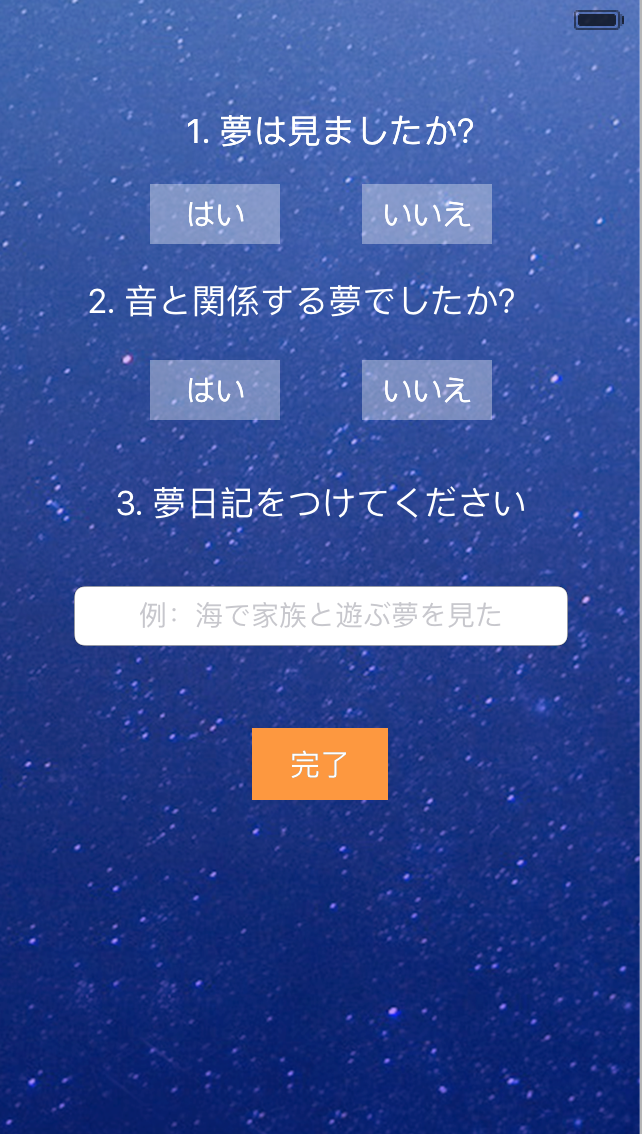
\includegraphics[height=90mm]{eps/AppDiary.eps}
  \end{center}
  \caption{夢日記記入ページ}
  \label{le05}
 \end{minipage}
 \begin{minipage}{0.45\hsize}
 \end{minipage}
\end{figure}

\section{システム概要:アプリの動作}
 Xcode 上で openframeworks ライブラリを利用して、iPhoneの加速度センサを利用した体動検知アプリケーションを制作した。睡眠時に枕の横に iPhone を置いて、体動(寝返り)による寝具の動きを検知して加速度を測定す る。\\

\subsection{キャリブレーション}
 まずベッドの硬さは人により違うため、キャリブレーションをする。アプリ起動後初めてDreamtravelerを使用するユーザーにはiPhoneを横に置いた状態で15秒間静止してもらう。x軸の加速度を毎秒記録、1病前の加速度との差分を導き出す。20秒間、x軸の差分の中での最大値を閾値として設定する。y軸とz軸の測定をしなかったのはx軸だけでも十分寝返りを特定できるためである。\\

\subsection{モニタリングと音楽再生}
 ベッドで寝てから睡眠に至るまで平均的に10分から20分かかるとされているため、スタートボタンが押されてから20分後に加速度センサーによる体動のモニタリングが開始される。モニタリングが開始されてからはノイズを除去するために、毎20秒の平均値が出される。その平均値が閾値に比べて高くなった時に寝返りをしたと判定する。寝返りを打つ時は睡眠段階がREM睡眠からnonREM睡眠に、あるいはnonREM睡眠からREM睡眠への切り替わったときだ\cite{negaeri}。そのためREM睡眠に突入した場合はあらかじめ設定していた音楽が図\ref{melodyGraph}のように流れる。

\begin{figure}[htbp]
\begin{center}
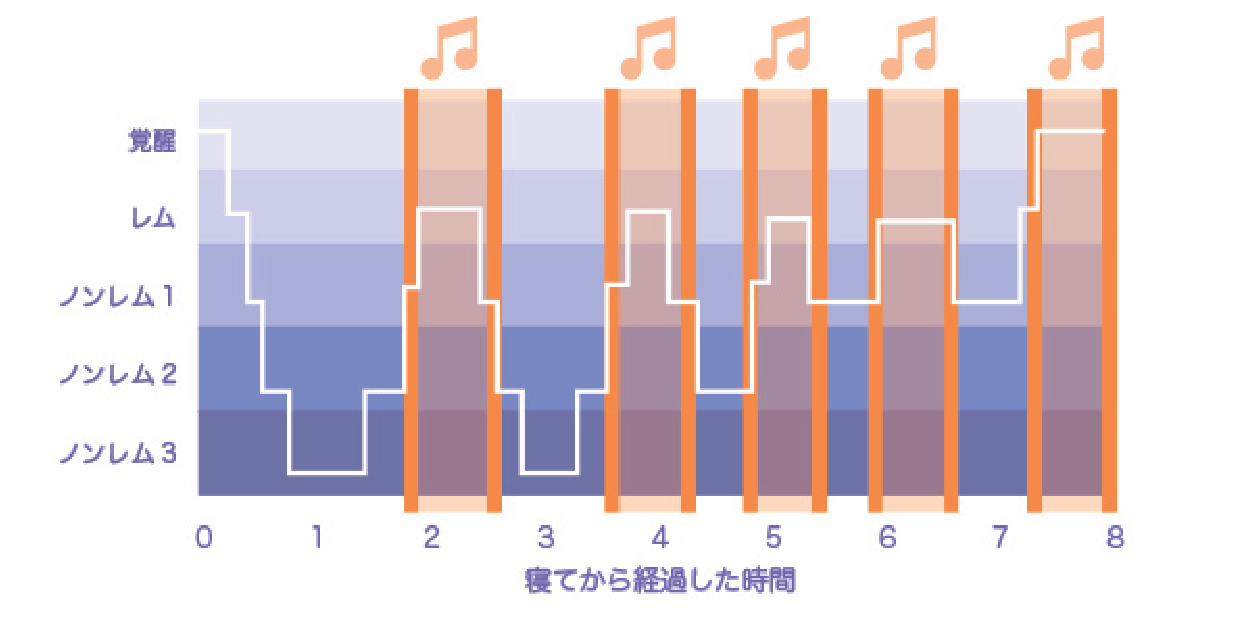
\includegraphics[width=15cm]{eps/remNonrem.eps}
\caption{ノンレムとレム睡眠}
\label{melodyGraph}
\end{center}
\end{figure}


\subsection{記録}
一晩中のx軸の数値、音楽の再生状況、夢日記の結果はデータベースをクラウドであるParseに保存する。図\ref{system}に一連のプログラムの流れを記載する。

\begin{figure}[htbp]
\begin{center}
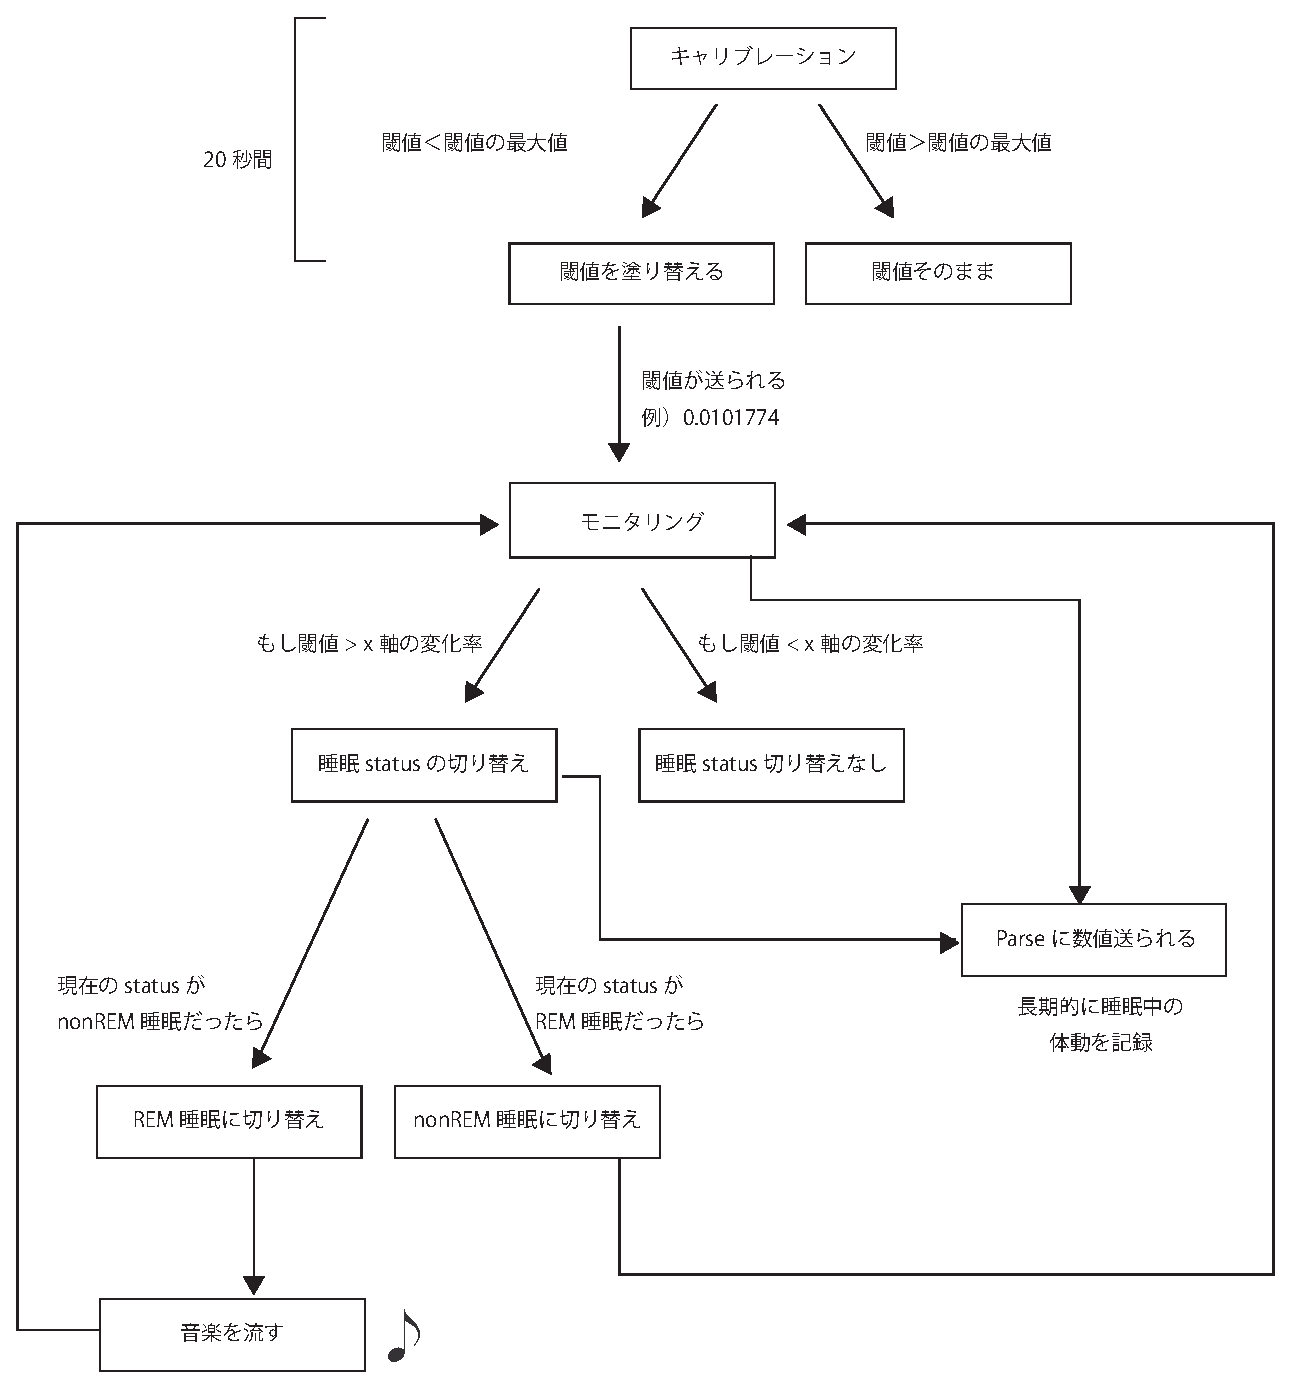
\includegraphics[width=12cm]{eps/system.eps}
\caption{Dreamtravelerのシステム}
\label{system}
\end{center}
\end{figure}

以下の図はDreamtravelerのセンシング結果を他のアプリケーションと比較したものだが、非常に近いデータの結果が出たことがわかる。それらのjsonデータをcsvデータに置き換えて、グラフ化したものと※〜〜〜ここに図を入れる。

%\begin{figure}[htbp]
%\begin{center}
%\includegraphics[width=10cm]{eps/sensing.eps}
%\caption{センシング部分の他のアプリとの比較}
%\label{sensing}
%\end{center}
%\end{figure}